\documentclass{beamer}
\usepackage[utf8]{inputenc}
\usepackage[T1]{fontenc}
\usepackage{graphicx}
\usepackage{multicol}
\graphicspath{{./images/}}

\usetheme{Arguelles}

\title{Using FPGAs to Perform Cryptanalytic Attacks on Random Number Generators}
\subtitle{}
\date{27/5/2021}
\author{Andreas Stocker}
\institute{University of Nicosia\par\email{andreas@stockers.org}}

\begin{document}

  \frame[plain]{\titlepage}
  

  \begin{frame}
    \frametitle{Abstract}
    \framesubtitle{The purpose of this paper}

    This paper combines two somewhat unrelated subjects, FPGAs and cryptanalysis.
    It provides background on both of these subjects and then culminates
    in an experiment that combines the two.
  \end{frame}

  \Section{FPGAs}

  \begin{frame}
    \frametitle{What are FPGAs?}


    \begin{multicols}{2}

    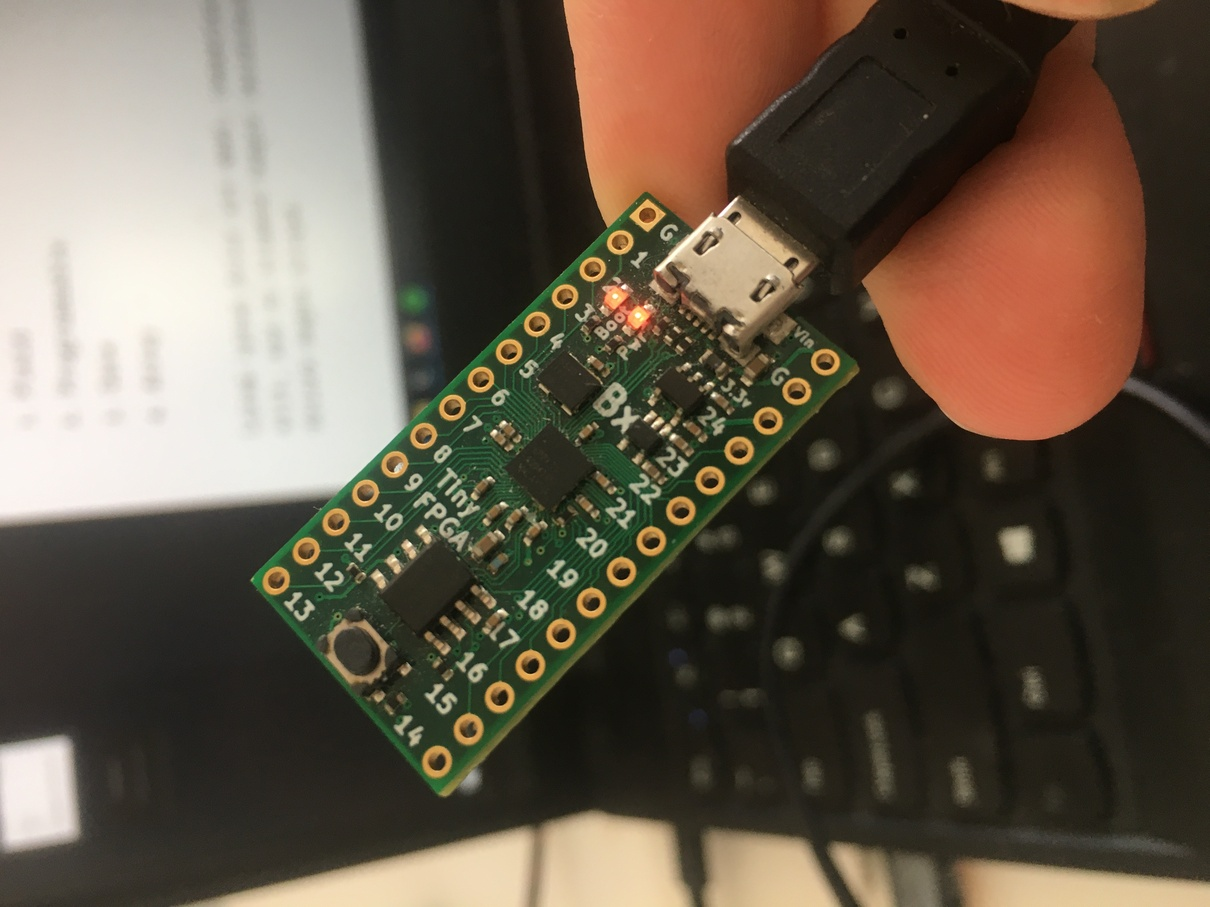
\includegraphics[scale=0.15,angle=-90]{tinyfpga-bx}
    
    \vfill
    
    \vspace*{\fill}
    
    \AlegreyaExtraBold FPGA \ttfamily stands for:
    \begin{enumerate}
      \item Field
      \item Programmable
      \item Gate
      \item Array
    \end{enumerate}
    
    \vspace*{\fill}

    \end{multicols}
    
  \end{frame}
  
  \begin{frame}
    \frametitle{FPGA Core Components}
    FPGAs are composed of the following \textit{core components}:
    \begin{itemize}
      \item Programmable Logic Blocks (PLBs)
      \item Specialized Logic Blocks
      \item Routing
      \item Clocks
    \end{itemize}
  \end{frame}
  
  \begin{frame}
    \frametitle{FPGAs verses ASICs}
    \framesubtitle{What are ASICs?}

    \textit{ASICs} are "Application Specific Integrated Circuits".

    \vfill

    CPUs for example are one of many types of ASICs.

    \vfill

    ASICs are produced through a silicon etching process that
    involves shining light through a mask and onto a photosensitive substance.

  \end{frame}
  
  \begin{frame}
    \frametitle{FPGAs verses ASICs}
    \framesubtitle{How do ASICs differ from FPGAs}

    Like the name suggests, FPGAs are \textit{field programmable}. \\
    This means the circuit of an FPGA can be quickly reconfigured.

    \vfill

    ASICs cannot be reconfigured and their circuit structure
    is set in stone from the time they were manufactured.

    \vfill

    Technically speaking, FPGAs themselves are a type of ASIC.

    \vfill

    There are numerous pros and cons that arise from these properties.

  \end{frame}

  
  \begin{frame}
    \frametitle{FPGAs verses ASICs}
    \framesubtitle{Where ASICs Shine}

    The static nature of ASICs brings a number of advantages.

    \vfill
    
    \begin{itemize}
      \item Cheaper to \textit{mass produce}
      \item More energy efficient
      \item Higher performance
      \item More compact
    \end{itemize}

  \end{frame}

  \begin{frame}
    \frametitle{FPGAs verses ASICs}
    \framesubtitle{Where FPGAs Shine}

    \AlegreyaSansMedium While ASICs have the upper hand in most categories, FPGA's have
    one essential advantage:

    \vfill
    
    \AlegreyaBlack It's far easier to modify an FPGA's design than an ASIC's.
    
    \vfill
      
    \AlegreyaSansMedium Developing and producing an ASIC design can cost \AlegreyaBlack
    millions of dollars. \\
    
    \vfill
    
    \AlegreyaSansMedium Producing a mask alone is extremely expensive. \\
    The designers cannot afford to make any mistakes. \\

  \end{frame}

   
  \ThankYou
  \begin{frame}[plain,standout]
    In combination with \textit{plain},\par
    it makes a nice thank-you slide!

    \vfill{Generated using \textit{Beamer} and the \textit{Arguelles} Theme}
  \end{frame}

\end{document}
